%%%%%%%%%%%%%%%%%%%%%%%%%%%%%%%%%%%%%%%%%
% Journal Article
% LaTeX Template
% Version 2.0 (February 7, 2023)
%
% This template originates from:
% https://www.LaTeXTemplates.com
%
% Author:
% Vel (vel@latextemplates.com)
%
% License:
% CC BY-NC-SA 4.0 (https://creativecommons.org/licenses/by-nc-sa/4.0/)
%
%%%%%%%%%%%%%%%%%%%%%%%%%%%%%%%%%%%%%%%%%

%----------------------------------------------------------------------------------------
%	PACKAGES AND OTHER DOCUMENT CONFIGURATIONS
%----------------------------------------------------------------------------------------

\documentclass[
	a4paper,
	10pt,
	unnumberedsections,
	twoside,
]{research_article}

\runninghead{Blood Smear Image Machine Learning Interpretability}

\footertext{\textit{}}

\setcounter{page}{1}

%----------------------------------------------------------------------------------------
%	TITLE SECTION
%----------------------------------------------------------------------------------------

\title{Methods for Interpreting Machine Learning Techniques in Blood Smear Image Based Leukaemia Classification}

\author{Aiden Abignano\textsuperscript{1}, Dr. Hesam Hesamian\textsuperscript{1} and Dr. Mukesh Prasad\textsuperscript{1}}

\date{\footnotesize\textsuperscript{\textbf{1}}University of Technology Sydney}

\renewcommand{\maketitlehookd}{
	\begin{abstract}
		\noindent Leukaemia diagnosis requires timely and accurate methods. This research explores the implementation of machine learning models using blood smear images to enhance diagnostic accuracy. Deep learning architectures like VGG, ResNet, and DenseNet are trained and compared, evaluating precision, sensitivity, specificity, and the F1 score. To address the interpretability challenge, techniques such as Grad-CAM, LIME, and shapley values are incorporated, providing insights into the models' decision-making processes. By combining accuracy assessment with interpretability analysis, this study aims to improve transparency, trust, and understanding in healthcare decision support systems and contribute more reliable diagnostic tools, facilitating early detection and prompt treatment of Leukaemia, thereby enhancing patient outcomes.
	\end{abstract}
}

%----------------------------------------------------------------------------------------

\begin{document}

\maketitle % Output the title section

%----------------------------------------------------------------------------------------
%	ARTICLE CONTENTS
%----------------------------------------------------------------------------------------

\section{Introduction}

Leukaemia is a form of blood cancer affecting white blood cells. During the production of new white blood cells, there are rare instances that can lead to the development of a blast cell which is an immature cell which has not been fully developed. While a single blast cell itself is not problematic, a large influx of blast cells can lead to Leukaemia as they are produced in such quantities that overwhelm the development of healthy blood cells and interfere with their established functions. Over time, as the remaining healthy cells age and need to be replaced, only these malignant cells are produced replacing the existing healthy blood cells eventually becoming the dominant white blood cell. Since white blood cells are responsible for fighting infection, Leukaemia can lead patients vulnerable to other diseases. Furthermore, as these cells circulate the blood stream they are capable of causing catastrophic harm to other internal organs such as the spleen, liver, kidneys and brain. For this reason, early treatment is the biggest factor in the success of a patient's recovery making early detection one of the most critical aspects in ensuring a favourable outcome.

Presently, Leukaemia is diagnosed by highly skilled medical practitioners manually analysing blood smear images and bone marrow extracts gathered from the patient, meticulously assessing the proportion of healthy white blood cells and cancerous ones. This procedure is extremely time consuming, highly labourios and prone to human errors leading to further delays in the necessary treatment and in some extreme cases false diagnoses. Moreover, this operation can also be taxing on the medical industry as qualified staff will often perform multiple roles in hospitals which cannot be easily replaced, making this time consuming diagnosis more troubling.

As machine learning algorithms have matured, there has been a growing interest by researchers to probe the possibility of such an algorithm capable of diagnosing Leukaemia with at least the same correctness of current medical staff, if not more. Such an algorithm would significantly reduce the time for diagnosis, especially in remote communities which do not have access to staff directly, and need to send blood smear images to foreign hospitals for inspection. While the current technology is promising, contemporary models still aren't reliable enough to completely automate the diagnosis process without human oversight to verify the results, making the technology moot.

After in-depth analysis of the present research, it is clear there are still research gaps that have held the technology back. multiple different types of models have been trained and compared including deep learning ones such as VGG, ResNet and DenseNet but a common issue noted between the papers is that, while the models themselves are capable of being highly accurate, they are still "black boxes" which lacks any insight into how the output has been reached. This has made it hard to integrate these models into the current diagnosis process as neither medical practitioners or patients have faith in their results.

There has been a growing interest in model interpretability, which addresses these shortcomings, due to its potential benefits in enhancing trust and understanding of the models. Interpretable models offer transparency, allowing healthcare professionals to comprehend and explain the reasoning behind the model's predictions. This understanding can significantly improve the adoption and acceptance of AI systems in medical settings, as clinicians can gain insights into how the model arrived at its conclusions. Interpretability also enables the identification of relevant features and patterns that contribute to diagnoses, empowering medical experts to make informed decisions and potentially uncover new medical insights. By embracing model interpretability, medical diagnosis models can bridge the gap between AI and human expertise, paving the way for more accurate, accountable, and reliable healthcare decision support systems.

This report will explore the implementation of machine learning models for diagnosing Leukaemia through blood smear images and evaluate their accuracy by considering multiple factors including accuracy, precision, sensitivity, specificity and F1 score. Additionally, this report will investigate different interpretability techniques which will be incorporated into the models including gradient-weighted class activation maps (Grad-CAM), local interpretable model-agnostic explanations (LIME) and shapley values to gain a deeper understanding of the models' inner workings. By combining accuracy assessment with interpretability, a comprehensive analysis of the models' performance and their underlying decision-making processes will be conducted. This approach not only focuses on achieving high predictive performance but also strives to provide insights into how the models arrive at their conclusions. Ultimately, this integrated approach will contribute to a more holistic evaluation of machine learning models, enabling better-informed decisions and fostering transparency in their applications. This report will cover the research aims and objectives, along with the significance and importance of the research, and the methods that will be used to ensure a fair and accurate study.

%------------------------------------------------

\section{Literature Review}
After further reading each source and comparing them with each other and back to the original intention of this literature review. It is clear there are several areas where the papers differ and where they are similar. This includes areas such as the models assessed, how the models have been modified, datasets trained on, preprocessing methods, results assessment and the goals of the conducted research. By reviewing these papers within the context of each other it is possible to understand common research gaps and inform future research which this paper will build from.

\pagebreak
The first study developed a comprehensive dataset comprising 3562 peripheral blood smear (PBS) images sourced from 89 patients, including both healthy individuals and patients definitively diagnosed with ALL subtypes. This dataset stands out for its inclusivity of benign cases, providing a realistic scenario for model training and subclassifies the form of Leukaemia diagnosed including Early Pre-B, Pre-B, and Pro-B ALL. In their methodology, the team employed ten well-known CNN architectures, such as EfficientNet, MobileNetV3, VGG-19, and DenseNet201, for feature extraction. Among the top performing models included DenseNet, InceptionResNetV2 and VGG-16 achieving 99.85\%, 99.54\% and 98.02 respectively. Notably, DenseNet201 emerged as the most effective model, yielding an accuracy of 99.85\%, a sensitivity of 99.52\%, and a specificity of 99.89\%. This high performance underlines the potential of CNNs in enhancing diagnostic accuracy and reducing misdiagnosis risks.

Attention maps were also added to the final model to highly regions of interest that had the most influence on the model's outcome. While this does add a layer of interpretability to the model, it was not the focus of the paper and since the dataset used was of full blood smear images, the attention maps provided vague heat maps highlighting large parts of the image rather than individual cells/regions as is desired.

The second study is a collection of papers presented as part of the C-NMC challenge. This challenge engaged 251 teams of researchers, leveraging a dataset of 15,114 cell images divided into training and testing sets. A variety of pre-trained deep learning models were modified and assessed, including VGG16, ResNet18, and the DenseNet series. Notable results included VGG16 achieving a 0.9175 validation score and 0.9171 weighted F1 score, ResNet18 reaching a 0.859 weighted F1-Score, and various DenseNet models displaying validation accuracies between 80.90\% and 81.58\%. Additionally, one paper reported a high validation accuracy of 92.48\% with AlexNet. The papers in this collection detailed the process and methodologies employed by contestants in developing their models. A key takeaway from these findings was that more complex models did not necessarily yield better accuracy, as evidenced by similar or even lower performance metrics compared to their less complex counterparts. This outcome underscores the significance of model optimization and selection in medical image analysis, challenging the preconception that increased model complexity invariably leads to superior results.

This study is based on the C-NMC challenge dataset presenting a novel architecture, SDCT-AuxNet$\theta$, for classifying ALL cell images. This two-module framework combines a compact CNN and a Kernel SVM, utilising bilinear-pooling features and spectral-averaged features, respectively. The study also proposes a novel testing strategy that uses confidence scores from both classifiers for decision-making. This method achieved a weighted F1 score of 94.8\% which is among the top performers for this dataset.

The third study uses a more custom designed model introducing an innovative approach using a Bayesian-optimised convolutional neural network (CNN) for the detection of ALL in microscopic smear images. The researchers also used a hybrid dataset which amalgamates two public ALL datasets; ALL-IDB1 and ALL-IDB2. The ALL-IDB1 subset comprises full blood smear images with accompanying textual files providing the (X,Y) coordinates of the blast cells' centroids. This subset contains a total of 108 images, split into 59 healthy and 49 diseased images. The ALL-IDB2 subset consists of images of individual cells rather than whole blood smear images with 260 images equally divided between healthy and diseased classes. By integrating these subsets, the study constructs a robust dataset of 368 blood smear images, providing a balanced representation of both healthy and ALL-diseased cases. This dataset underpins the study's Bayesian optimization approach, where the CNN's architecture and hyperparameters are meticulously fine-tuned to the specific characteristics of the data. This method leads to a marked improvement in the performance of image-based ALL classification, illustrating the potential of custom-tailored machine learning models in the precise and reliable diagnosis of medical conditions like ALL.

As using deeper models does not necessarily lead to more accurate models, there has been a focus on using other methods such as highly custom models, transfer learning, and various preprocessing techniques to improve results. The focus of this research will be toward exploring the efficacy of transfer learning with pre-trained models along with various preprocessing techniques. This approach aligns with the strategies employed by the majority of contestants in a previous study, the C-NMC challenge, where pre-trained models were adapted and fine-tuned for similar diagnostic tasks. Emphasising transfer learning acknowledges the practical benefits of leveraging existing, well-established models, which can be more accessible and efficient.

\newpage
As Grad-CAM, LIME and shapley values are being implemented for the interpretability part of this research, their respective papers have also been reviewed.

Grad-CAM is used to understand the regions of an image that contribute most to the network's decision-making process. By analysing the gradients that flow into the final convolutional layer of the CNN, Grad-CAM generates a heat map that highlights the important regions of the input image. This heat map indicates the areas that the CNN focuses on when making predictions, visually revealing features that the model considers most relevant allowing us to understand which image regions drive its decisions.

LIME focuses on understanding the model's behaviour on an individual prediction basis. It does this by perturbing the input image, generating numerous variants, and observing how these alterations impact the model's output. By examining these changes, LIME identifies the regions and features of the input image that are most influential in the model's decision-making process. This local interpretation provides insights into which specific aspects of the image drive the prediction, thereby offering a clearer understanding of the model's reasoning on a case-by-case basis. The method is particularly useful for highlighting the localised features and regions that contribute significantly to individual predictions, thereby demystifying the model's operation at a granular level.

SHAP provides insights into the individual contributions of input features in a CNN by quantifying the importance of each feature by assigning a Shapley value, which represents the average marginal contribution of a feature across all possible feature combinations. SHAP helps in understanding the impact of each feature on CNN's predictions by decomposing the prediction into the contributions from each input feature. This allows attributing the model's output to specific features and assessing their significance. By analysing the SHAP values, a deeper understanding of the relative importance and influence of different features on CNN's decision-making process is gained. 

These studies collectively demonstrate the crucial role of dataset creation, model selection, and optimization in medical diagnostics. The development of specialised datasets, like the one in the first study, provides a robust foundation for training and testing models. The insights from the C-NMC challenge and the Bayesian-optimised CNN approach further highlight the importance of choosing and fine-tuning the right model to achieve high accuracy and reliability in medical imaging diagnostics, particularly in the context of ALL. Furthermore, the role of interpretability has been highlighted for its ability to gain a deeper understanding in model insights and effectiveness and the ways different interpretability models vary and what they do and don't show. The advancements in these areas not only enhance diagnostic precision but also contribute significantly to the trust and acceptance of AI systems in medical settings.

%------------------------------------------------

\section{Research Aims and Objectives}

The primary aim of this research is to explore the implementation of machine learning models for diagnosing Leukaemia using blood smear images and to evaluate their accuracy through various performance metrics. The objective is to develop robust and reliable machine learning models that can accurately distinguish between healthy white blood cells and cancerous ones. By leveraging the power of machine learning algorithms, the research aims to reduce the time-consuming and error-prone manual analysis currently performed by highly skilled medical practitioners. The ultimate goal is to develop an automated diagnostic tool that can provide quick and accurate diagnoses, particularly benefiting remote communities with limited access to medical staff and facilities. This will include a range of machine learning methods including VGG(16 and 19), ResNet(50 and 101) and DenseNet(121 and 169). After training the models, multiple well-established quantitative measurements including accuracy, precision, sensitivity, specificity and F1 score will be made to assess the ability of each model.

Additionally, the research seeks to address the lack of interpretability in contemporary machine learning models. The objective is to incorporate interpretability techniques such as gradient-weighted class activation maps (Grad-CAM), partial dependence plots, and shapley values into the models which will analyse and graph various insights of the model in a way humans can understand. By doing so, the research seeks to provide transparency and understanding regarding the models' decision-making processes. This will enable healthcare professionals to comprehend and explain the reasoning behind the models' diagnostic predictions, enhancing trust and acceptance of AI systems in medical settings. The research also endeavours to identify relevant features and patterns contributing to Leukaemia diagnosis, potentially leading to new medical insights and discoveries.

\newpage
The integrated approach of evaluating accuracy while incorporating interpretability will provide a comprehensive analysis of the machine learning models' performance. By combining quantitative performance metrics with qualitative insights into the models' inner workings, the research will contribute a more holistic evaluation of these models. While the focus for many previous researchers has been to create a model capable of replacing medical experts entirely in the diagnosis process by creating a model more accurate than them, this research aims to create a tool that complements their expertise and decision-making process through the use of interpretability. These interpretable models will also allow for comparing machine learning models in more nuanced ways  such as how much of the data is actually being considered and what patterns/trends it has found.

%------------------------------------------------

\section{Methodology}

Recent approaches in medical imaging analysis have primarily focused on creating models that assess blood smear images in their entirety. However, the objective of the proposed model diverges from this trend; it aims to enhance interpretability by classifying individual areas within an image. This refined approach requires the utilisation of two distinct datasets.

\subsection{Dataset Description and Rationale}

The primary dataset employed in this study is the "C\_NMC\_2019 Dataset," which has been used for training the classification model. This is a binary dataset comprising images of cancerous and non-cancerous cells. The identification of immature leukemic blasts in contrast to normal cells is a formidable challenge due to their similar morphological features under microscopic examination. The dataset, originally designed for a competition, is extensive and segmented into three phases: training, preliminary testing, and final testing. The training set includes 10,661 cell images from 73 subjects, while the preliminary test set and final test set comprise 1,867 and 2,586 cell images respectively, from a combined total of 45 subjects. For the purpose of the model, these separate parts of the dataset have been amalgamated into one comprehensive training dataset. The choice of this dataset is further justified by its substantial size and the diversity of high-accuracy models previously developed for it, providing a wealth of existing literature and comparative data.

\begin{table}[ht]
	\caption{C\_NMC\_2019 Dataset}
	\centering
	\label{tab:datasets}
	\begin{tabular}{lccc}
		\multicolumn{4}{c}{Subjects} \\
		\hline
		\textbf{Attribute} & \textbf{Train} & \textbf{Preliminary} & \textbf{Final} \\
		\hline
		ALL & 47 & 13 & 9 \\
		Normal & 26 & 15 & 8 \\
		Total & 73 & 28 & 17 \\
		\hline
	\end{tabular}
\end{table}

\begin{table}[ht]
	\caption{C\_NMC\_2019 Dataset}
	\centering
	\label{tab:datasets}
	\begin{tabular}{lccc}
		\multicolumn{4}{c}{Cell Images} \\
		\hline
		\textbf{Attribute} & \textbf{Train} & \textbf{Preliminary} & \textbf{Final} \\
		\hline
		ALL & 7,272 & 1,219 & Unknown \\
		Normal & 3,389 & 648 & Unknown \\
		Total & 10,661 & 1,867 & 2,586 \\
		\hline
	\end{tabular}
\end{table}

\begin{tabular}{m{3.25cm} m{4cm} m{4cm}}
	\textbf{Healthy} & \textbf{ALL} \\
	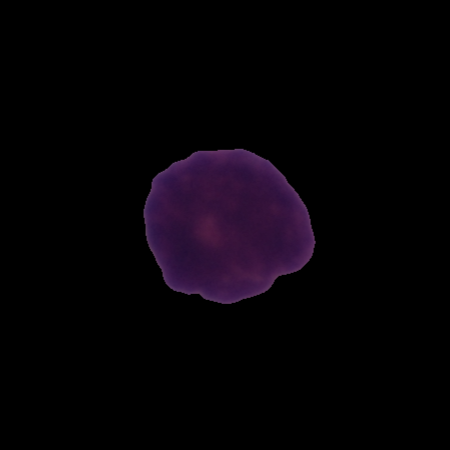
\includegraphics[width=3.5cm]{images/UID_H10_103_3_hem.png} & 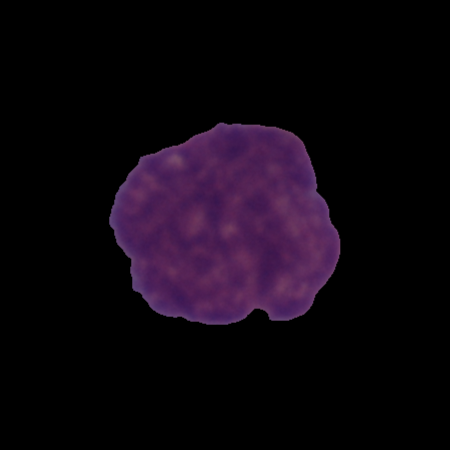
\includegraphics[width=3.5cm]{images/UID_11_16_2_all.png} \\
	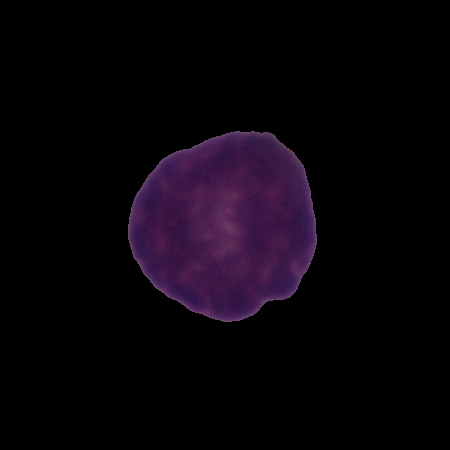
\includegraphics[width=3.5cm]{images/UID_H10_100_3_hem.png} & 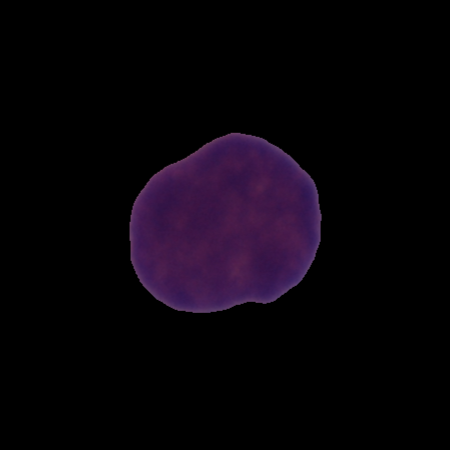
\includegraphics[width=3.5cm]{images/UID_11_2_1_all.png} \\
	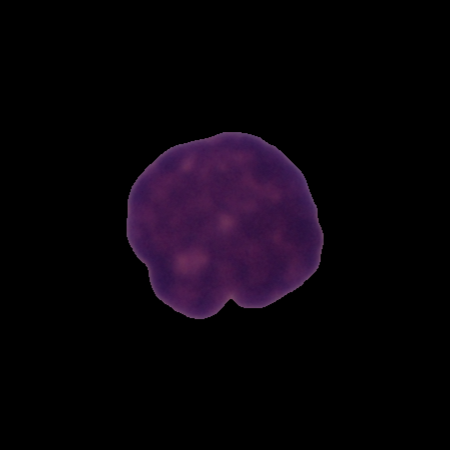
\includegraphics[width=3.5cm]{images/UID_H10_100_1_hem.png} & 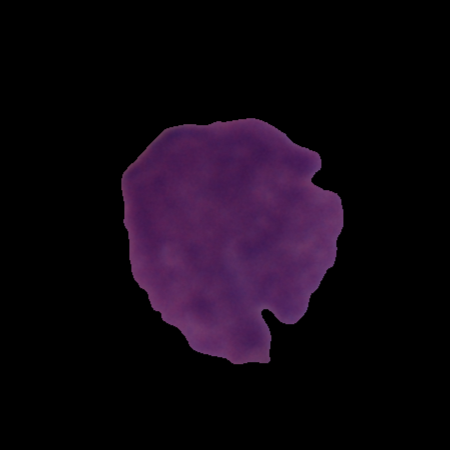
\includegraphics[width=3.5cm]{images/UID_11_10_1_all.png} \\
\end{tabular}

\subsection{Data Preparation and Preprocessing}

To prepare this dataset for the model, it has been split into training, validation, and testing phases with proportions of 64\%, 16\%, and 20\% respectively. As there is a significant imbalance in the dataset, with roughly double the number of healthy cells compared to cancerous ones, various balancing techniques have been employed. These include horizontal and vertical flipping and random rotations between 0 to 360 degrees. Additionally, image normalisation was achieved using calculated mean and standard deviation values. A significant challenge arose from the central positioning of cells in the images, which is not ideal when applied to the sliding windows of the second dataset. To mitigate this, additional black padding was introduced of various sizes on random sides of the image and centre cropped to shift the cell from its central position. The images, originally 450 x 450 pixels, were actually cropped to 448 x 448 in this process allowing the images to be downsized by a factor of two through max pooling, resulting in a final dimension of 224 x 224 pixels.

{\centering\textbf{Preprocessed Images}
\begin{tabular}{cc}
	
\includegraphics[width=3.5cm]{images/preprocessed_image1.png} & 
\includegraphics[width=3.5cm]{images/preprocessed_image2.png} \\
	\multicolumn{2}{c}{
\includegraphics[width=3.5cm]{images/preprocessed_image3.png}} \\
\end{tabular}
\par}

\subsection{Model Training and Evaluation}

In this study, the selection of deep learning architectures: ResNet (Residual Networks), DenseNet (Densely Connected Convolutional Networks), and VGG (Visual Geometry Group) was guided not only by their inherent capabilities but also by their demonstrated success in previous literature utilising the "C\_NMC\_2019 Dataset." These models have consistently emerged as top performers in medical imaging problems like blood smear classification. The ResNet architecture, acclaimed for its deep layers and residual connections, adeptly counters the vanishing gradient problem, facilitating the efficient training of deep networks. This is crucial for discerning subtle variances in blood cell imagery. DenseNet, with its unique dense connections, enhances feature propagation within the network, an essential trait for detailed examination of cellular structures. Meanwhile, VGG's deep convolutional layers excel in feature extraction from complex images, a vital function in distinguishing cancerous from non-cancerous cells. Moreover, This diversity in model sizes allows for a comprehensive evaluation of model performance across different architectural complexities, ensuring robustness and accuracy in classification.

\pagebreak
Each model will be modified with an added max pooling layer to downsample the 448 x 448 images into 224 x 224 ones. Furthermore the final output layer will be modified to have one output feature with a sigmoid function for mapping the values between 0 and 1 for binary classification. Each model will also start with pretrained ImageNet V1 weights provided by Pytorch.

An extensive training approach was adopted, running for 200 epochs with a patience of 20 to avoid overfitting, a batch size of five, and a learning rate of 0.001. The models were optimised using binary cross-entropy loss function and stochastic gradient descent. The evaluation of these models was based on a range of metrics, including accuracy, F1 score, recall, and precision. Additionally, the interpretability models, GradCAM++, LIME, and SHAP were applied to the testing part of this dataset to further analyse the model's decision-making process.
\newline\newline
\textbf{Accuracy}: Ratio of correctly predicted cases out of the total number of cases.
\begin{displaymath}
	Accuracy = \frac{True\ Positives + True\ Negatives}{Total\ number\ of\ cases}
\end{displaymath}

\textbf{Precision}: Ratio of correctly predicted positive cases to the total number of predicted positive cases. It tells us out of all the instances that were predicted as positive, how many were actually positive.
\begin{displaymath}
	Precision = \frac{True\ Positives}{True\ Positives + False\ Positives}
\end{displaymath}

\textbf{Recall (sensitivity)}: Ratio of correctly predicted positive cases to the total number of positive cases. High precision correlates to low false positive rate.
\begin{displaymath}
	Recall (sensitivity) = \frac{True\ Positives}{True\ Positives + False\ Negatives}
\end{displaymath}

\textbf{Specificity}: Ratio of correctly predicted negative cases to the total number of negative cases.
\begin{displaymath}
	Specificity = \frac{True\ Negatives}{True\ Negatives + False\ Positives}
\end{displaymath}

\textbf{F1 Score}: Harmonic mean of precision and recall, taking both false positives and false negatives into account. F1 score favours classifiers that have a similar precision and recall, which is especially useful in scenarios where an even balance between precision and recall is desired.
\begin{displaymath}
	F1 = 2 \times \frac{Precision \times Recall}{Precision + Recall}
\end{displaymath}

\newpage
\subsection{Secondary Dataset}
In addition to the primary dataset, a smaller dataset, ALL\_IDB1, was incorporated consisting of 108 high-resolution images of blood smears, captured using an optical laboratory microscope and a Canon PowerShot G5 camera. Each image is accompanied by a classification file indicating the centroids of probable ALL lymphoblasts. To analyse these full-scale blood smear images, a sliding window technique was employed with dimensions of 112 x 112 pixels and a step size of 56 pixels.

This window size was chosen to address a specific challenge encountered in the study: the first dataset, "C\_NMC\_2019," contains images with a single cell per image, whereas the ALL\_IDB1 dataset features multiple cells. To effectively analyse these more complex images without losing the focus on individual cells, it was crucial to find a balance between a window size large enough to encompass an entire cell and small enough to remove unwanted surrounding cells. 112 x 112 is also exactly half of the 224 x 224 pixel size used for the images in the primary dataset, facilitating more straightforward upscaling for the model. The choice of a 56-pixel step size for the sliding window, being half of the window dimension, was designed to reduce the instances of cells being split between two windows, while simultaneously avoiding an excessive increase in the number of windows needed for analysis. Any image containing the (x,y) coordinate of one of the blast cells were categorised as images containing cancerous cells and the rest were considered non-cancerous. Since the (x,y) coordinates were the centroid of the cell there will be cases where portions of cancerous cells are included in images marked as non-cancerous but never enough to affect the desired model outcome.

Similar to the primary dataset, these images underwent normalisation. The processed images were then fed into the classification model. Finally, the model's performance was further assessed using advanced evaluation techniques such as GradCAM++, LIME, and SHAP, alongside the metrics used for the first dataset.

\newpage
\begin{table}[ht]
	\caption{ALL-IDB1}
	\centering
	\label{tab:datasets}
	\begin{tabular}{lccc}
		\multicolumn{3}{c}{Images} \\
		\hline
		\textbf{Healthy} & \textbf{Diseased} & \textbf{Total} \\
		\hline
		59 & 49 & 108 \\
		\hline
	\end{tabular}
\end{table}


\noindent\begin{tabular}{c}
    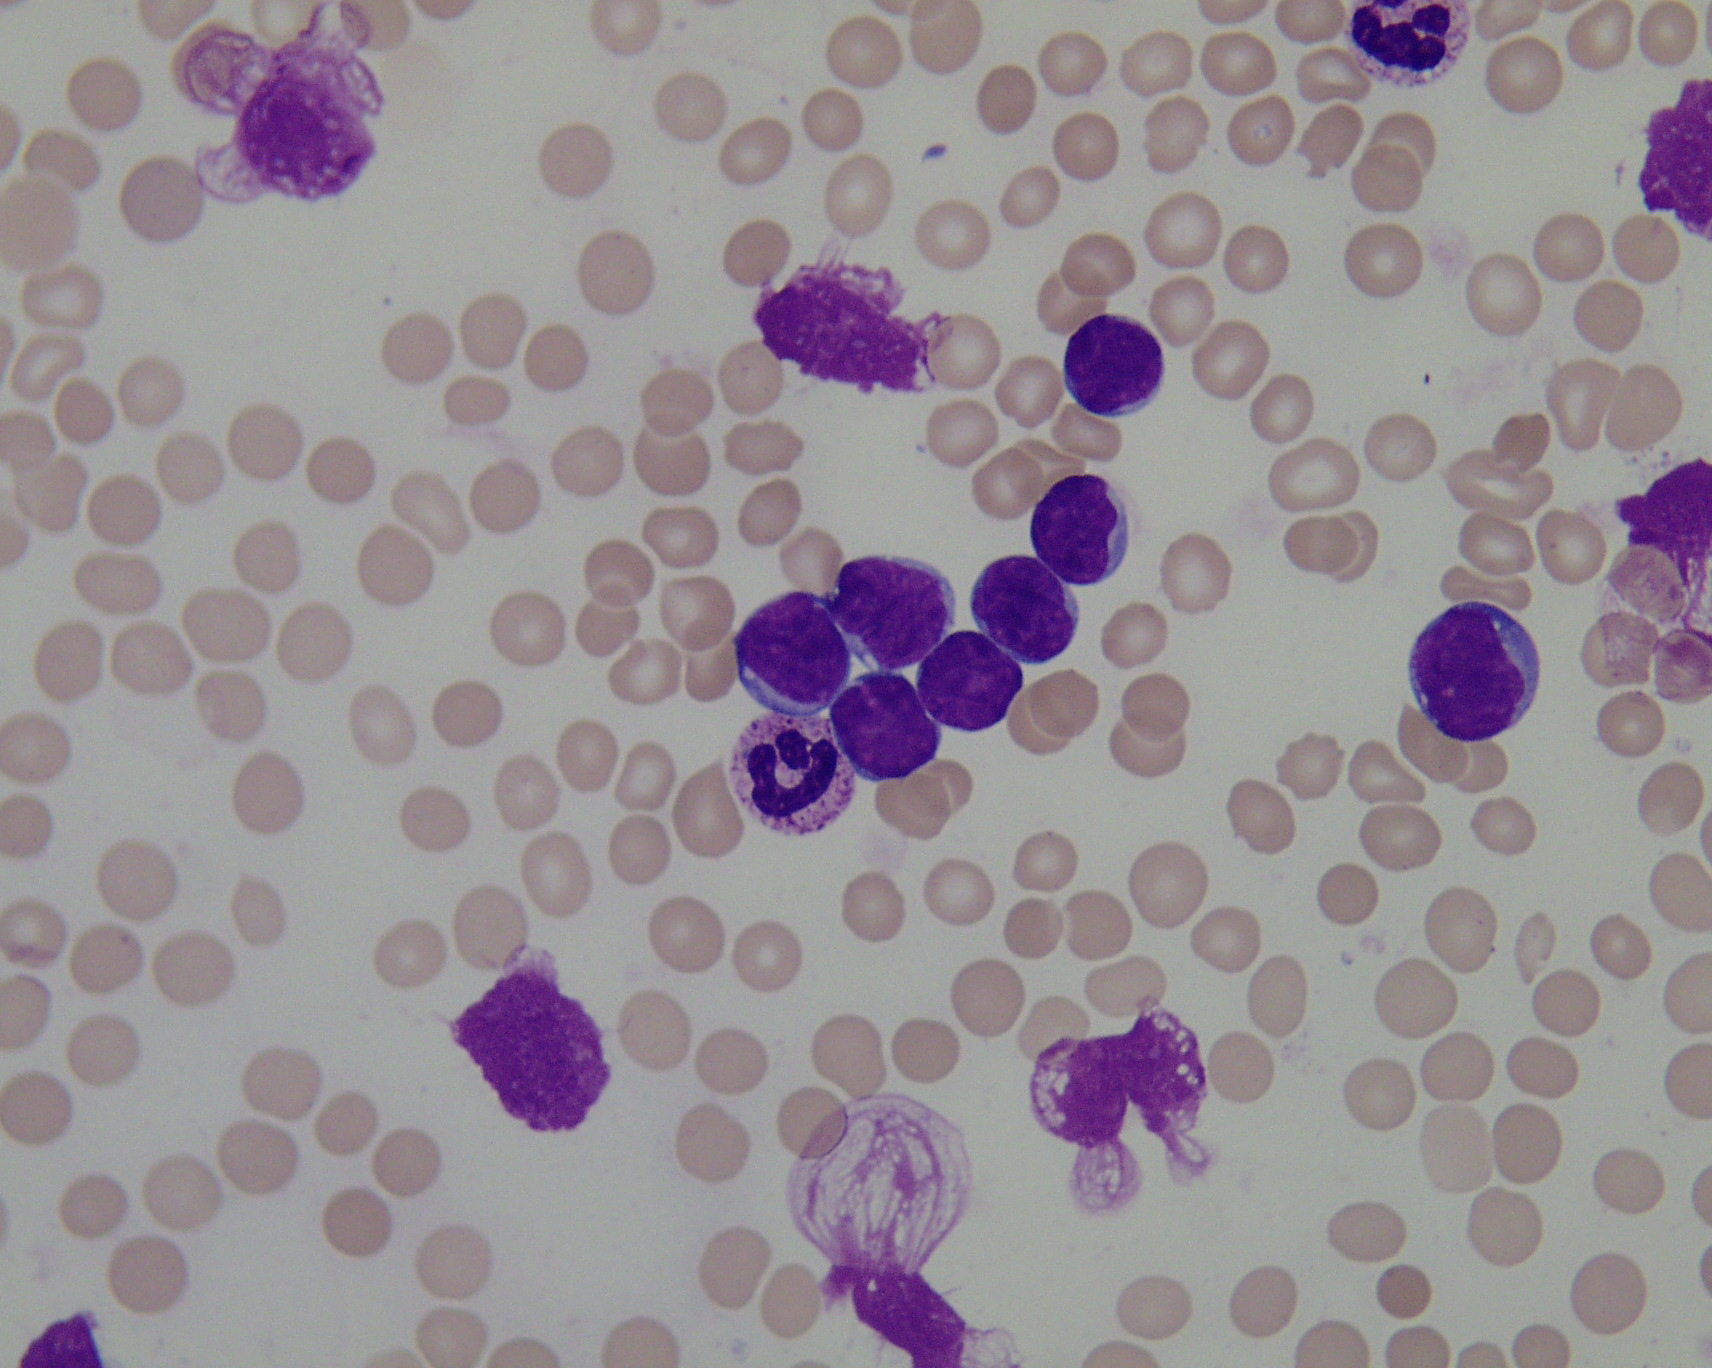
\includegraphics[width=\linewidth]{images/Im001_1.jpg} \\
    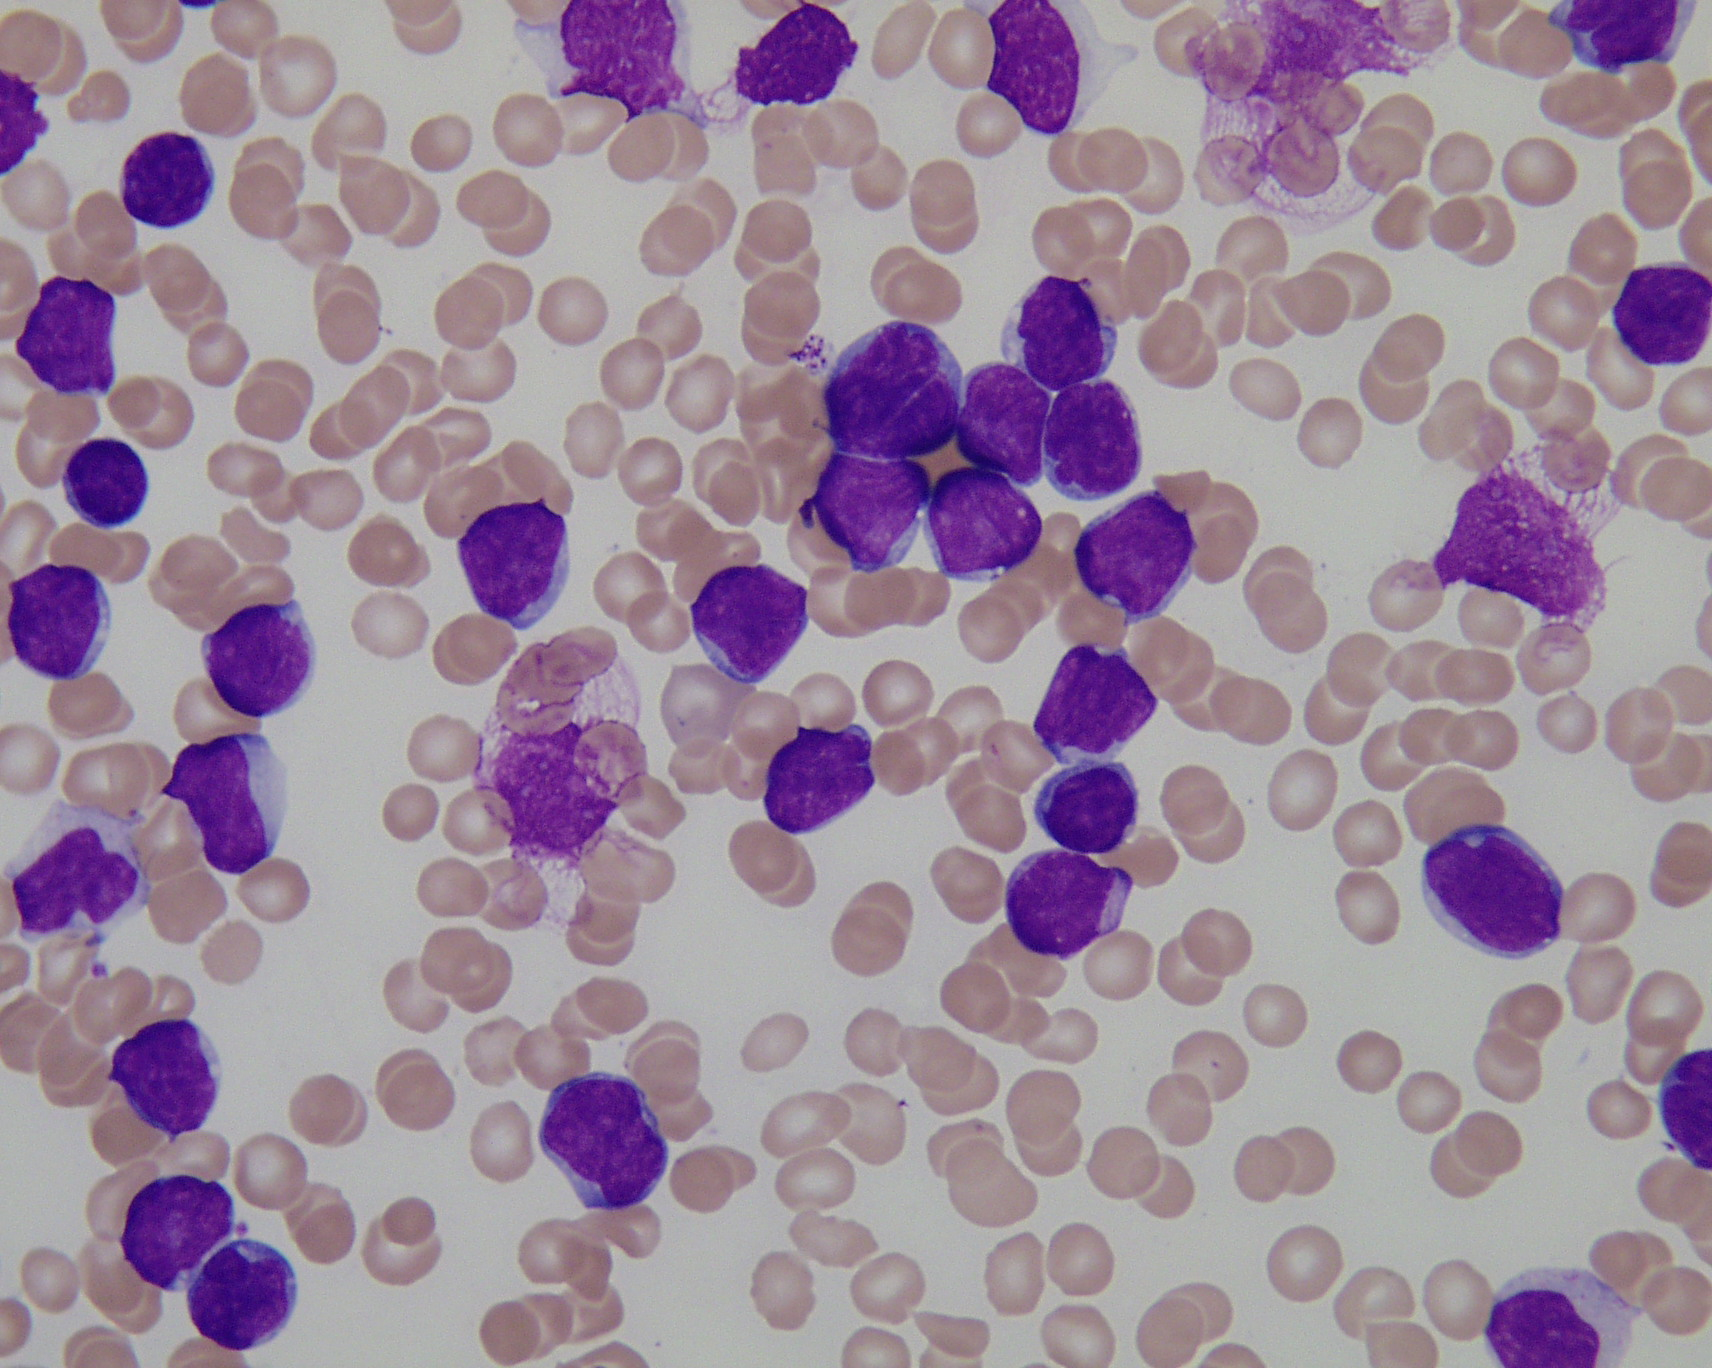
\includegraphics[width=\linewidth]{images/Im005_1.jpg} \\
    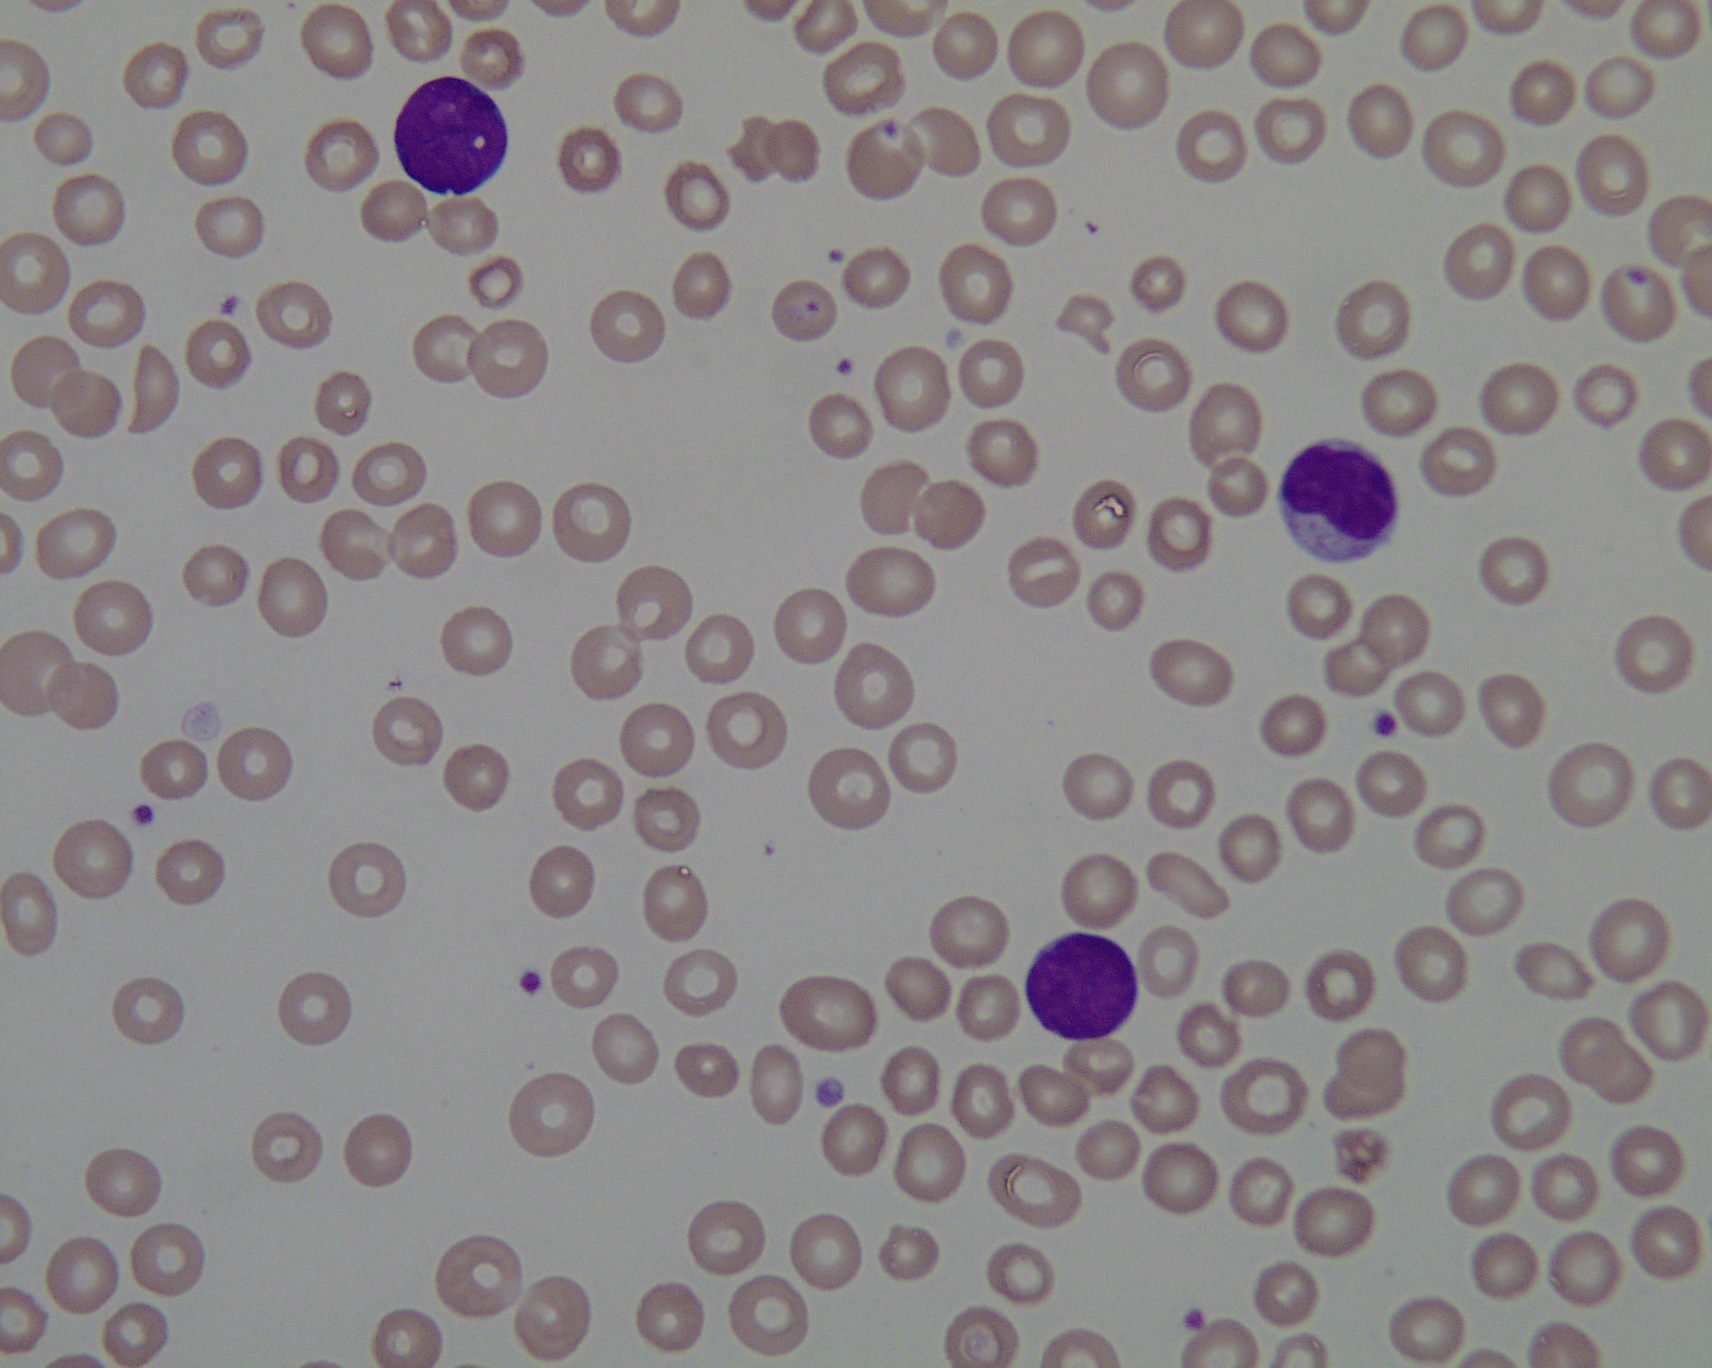
\includegraphics[width=\linewidth]{images/Im025_1.jpg} \\
\end{tabular}

\newpage
\begin{table}[ht]
	\caption{ALL-IDB1 Window Slides}
	\centering
	\label{tab:datasets}
	\begin{tabular}{lccc}
		\multicolumn{3}{c}{Images} \\
		\hline
		\textbf{Healthy} & \textbf{Diseased} & \textbf{Total} \\
		\hline
		55375 & 2539 & 57914 \\
		\hline
	\end{tabular}
\end{table}
\begin{tabular}{m{3.25cm} m{4cm} m{4cm}}
	\textbf{Healthy} & \textbf{ALL} \\
	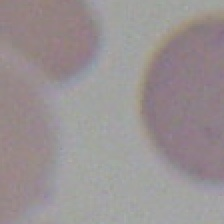
\includegraphics[width=3.5cm]{images/Im001_1_window_100.jpg} & 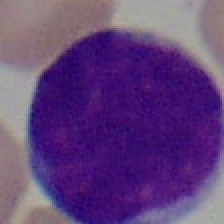
\includegraphics[width=3.5cm]{images/Im001_1_window_219.jpg} \\
	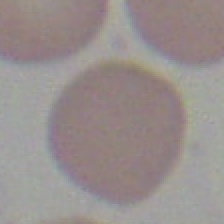
\includegraphics[width=3.5cm]{images/Im001_1_window_196.jpg} & 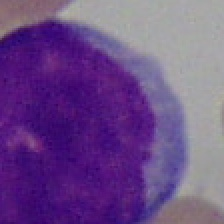
\includegraphics[width=3.5cm]{images/Im002_1_window_473.jpg} \\
	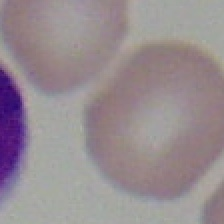
\includegraphics[width=3.5cm]{images/Im001_1_window_221.jpg} & 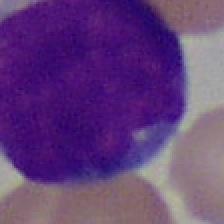
\includegraphics[width=3.5cm]{images/Im003_1_window_376.jpg} \\
\end{tabular}

%------------------------------------------------
\newpage\onecolumn
\section{Results}

\subsection{C\_NMC\_2019 Dataset}
\begin{table}[ht]
	\centering
	\begin{tabular}{lcccc}
		\hline
		\textbf{Models} & \textbf{Accuracy} & \textbf{Precision} & \textbf{Recall} & \textbf{F1 Score} \\
		\hline
		Resnet50    & 0.7732 & 0.7486 & 0.7970 & 0.7719 \\
		Resnet101   & 0.7901 & 0.7596 & 0.8179 & 0.7877 \\
		DenseNet121 & 0.8233 & 0.8245 & 0.8298 & 0.8271 \\
		DenseNet161 & 0.8303 & 0.8492 & 0.8250 & 0.8369 \\
		VGG16       & 0.9316 & 0.9369 & 0.9301 & 0.9335 \\
		VGG19       & 0.9189 & 0.9206 & 0.9189 & 0.9188 \\
		\hline
	\end{tabular}
\end{table}

These are the results calculated by running the models against the testing portion of the C\_NMC\_2019 dataset. In the comparative analysis of convolutional neural network architectures, the VGG16 model outperformed others, achieving the highest accuracy of 0.9316, precision of 0.9369, recall of 0.9301, and an F1 score of 0.9335. VGG19 followed closely, with a competitive performance showcasing an accuracy of 0.9189, albeit with marginally lower precision and recall rates. While the deeper models did perform slightly better than their less complex counterparts, they were still with 1-2 percent differences. Interestingly VGG16 managed to outperform VGG19 in every metric.

\newpage
\begin{center}
	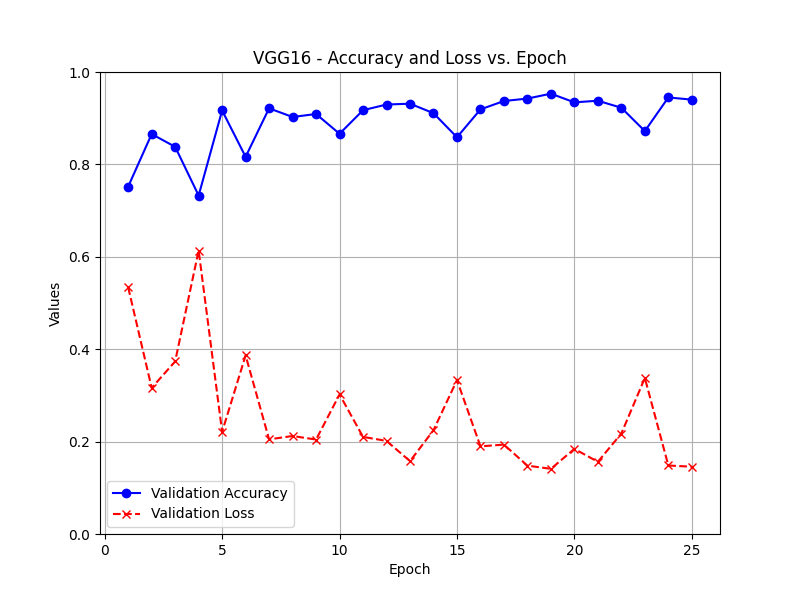
\includegraphics[width=0.89\linewidth]{images/vgg16_val_accuracy-lossVepoch.png}
	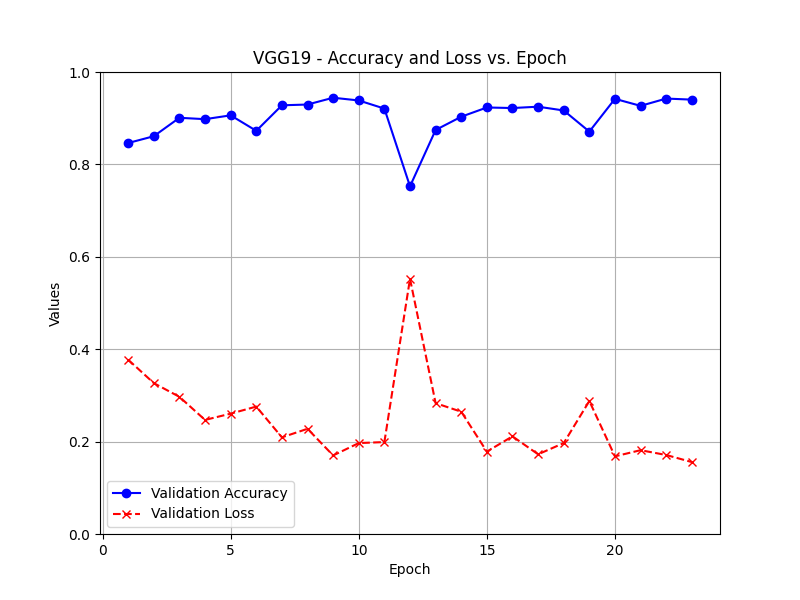
\includegraphics[width=0.89\linewidth]{images/vgg19_val_accuracy-lossVepoch.png}
\end{center}

These graphs show the validation accuracy and validation loss when training VGG16 and VGG19 respectively. They have been cut off at the epoch they reached their lowest loss value which was 25 and 23 respectively. This aligns with the results from other researchers training similar models on this dataset achieving their best results between epoch 20 to 30.

\newpage
These interpretability metrics were generated with the VGG16 model

\subsubsection{Grad-CAM}

\begin{center}
	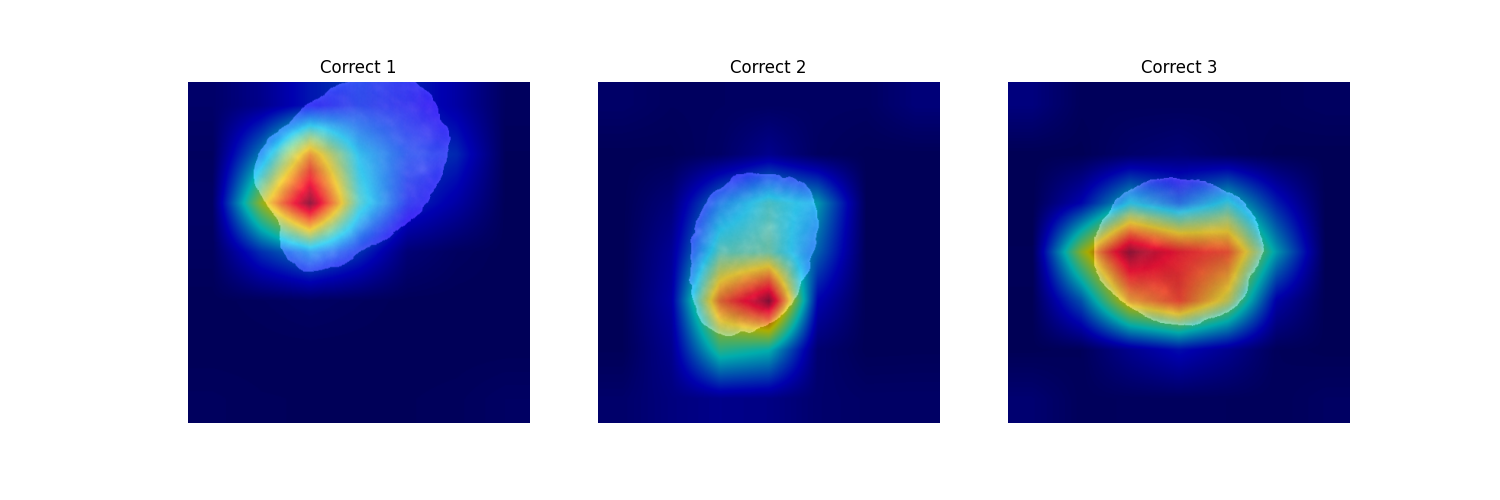
\includegraphics[width=\linewidth]{images/dataset1_gradcam_correct.png}
	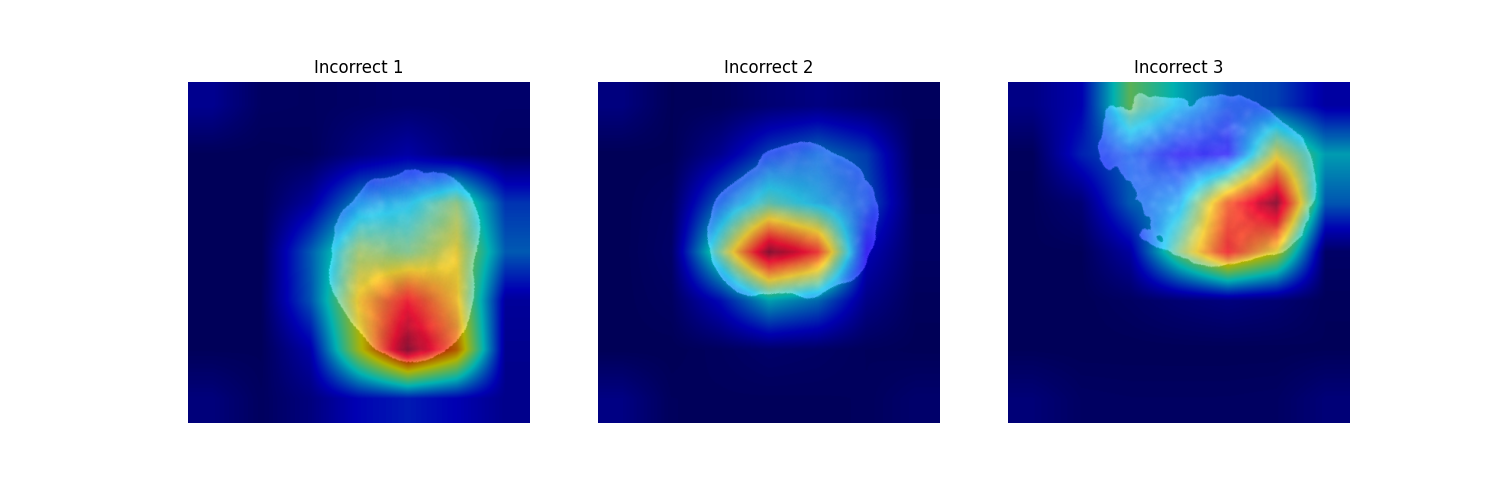
\includegraphics[width=\linewidth]{images/dataset1_gradcam_incorrect.png}
\end{center}

Here, a  heatmap is generated showcasing which areas in the image had the biggest impact on the model's outcome. Despite the second row of images being incorrectly predicted, it is clear the model is still focusing on important areas of the cell just as it does in its correct predictions.

\newpage
\subsubsection{LIME}

\begin{center}
	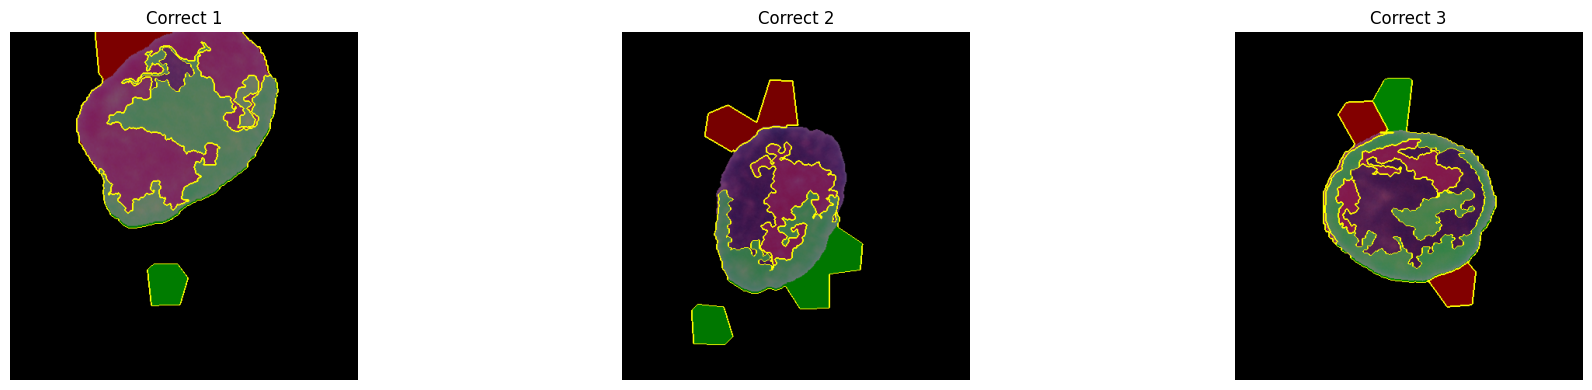
\includegraphics[width=\linewidth]{images/dataset1_lime_correct.png}
	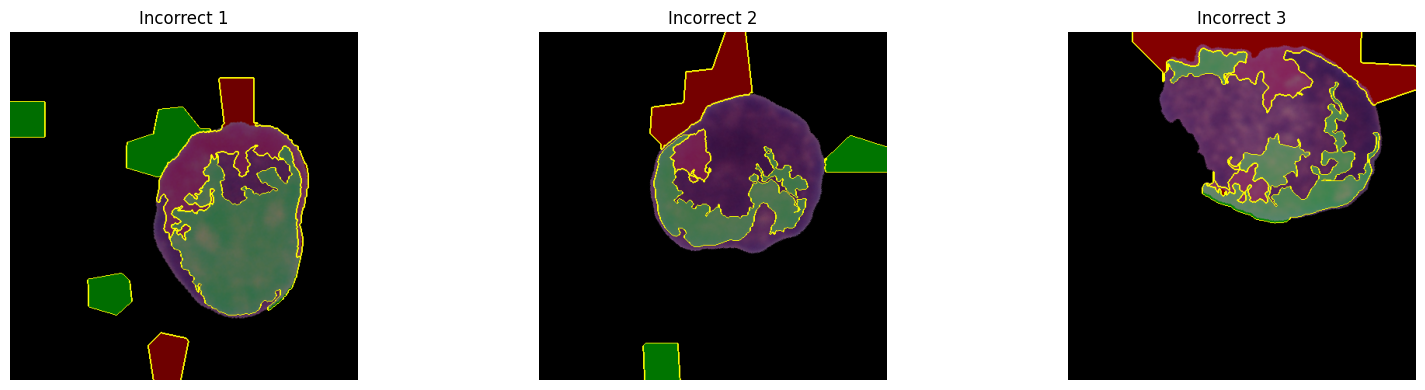
\includegraphics[width=\linewidth]{images/dataset1_lime_incorrect.png}
\end{center}

Here are the general LIME images. The green areas indicate the areas that contribute positively toward the model's prediction for a particular class and the red are regions that contribute negatively toward the model's prediction for the specified class. Here it can be seen the model seems to focus on areas outside the cell where the black padding is. This is especially intriguing as the background is solid black making those areas lack any noteworthy features. It does appear that where the model predicted incorrectly, it was focusing less on the cell compared to the correct predictions.

\newpage
\subsubsection{SHAP}

\begin{center}
	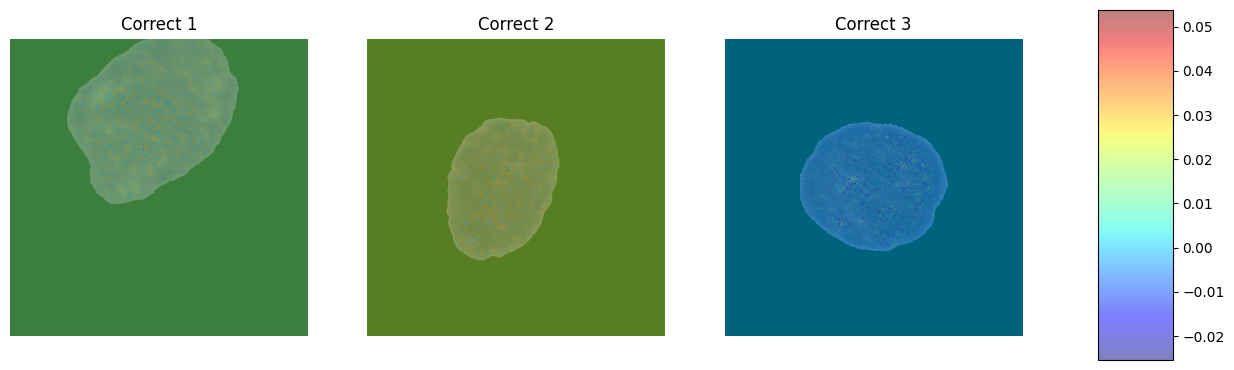
\includegraphics[width=\linewidth]{images/dataset1_shap_correct.png}
	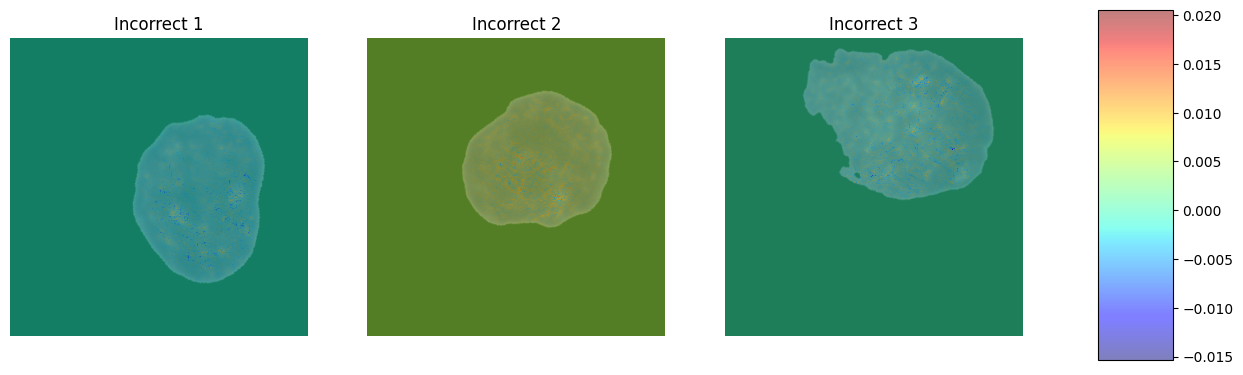
\includegraphics[width=\linewidth]{images/dataset1_shap_incorrect.png}
\end{center}

The generated shapley values are for each individual pixel of the image which is 448 x 448 each. The positive values (indicated in red) are features that push the model's prediction higher, and the negative values (indicated in blue) are features that push the model's prediction lower. A majority of the image is green as that is where 0 value is indicating more attention is being paid on the cell. Shapley values allow the ability to see the exact parts of the cell the model is using to determine its prediction. Similar to Grad-CAM, there is little difference between the correctly and incorrectly predicted images.


\newpage
\subsection{ALL-IDB1}

Since VGG was the most performant model. It was chosen to be applied to the second dataset.

\begin{table}[ht]
	\centering
	\begin{tabular}{lcccc}
		\hline
		\textbf{Models} & \textbf{Accuracy} & \textbf{Precision} & \textbf{Recall} & \textbf{F1 Score} \\
		\hline
		VGG16 & 0.7435 & 0.9432 & 0.7435 & 0.8188 \\
		VGG19 & 0.9189 & 0.9206 & 0.9189 & 0.9188 \\
		\hline
	\end{tabular}
\end{table}

These are the results from running the models trained on the first dataset on the entirely of the sliding windows derived from the ALL-IDB1 dataset. Notably, despite VGG16 performing better in the first dataset, the deeper model managed to outperform it by a significant margin. Specifically, VGG19 achieved an accuracy of 0.9189, precision of 0.9206, recall of 0.9189, and an F1 score of 0.9188. In contrast, VGG16 demonstrated lower efficacy with an accuracy of 0.7435, despite a notably high precision of 0.9432, which did not proportionally translate to recall, mirroring the accuracy at 0.7435, and culminating in an F1 score of 0.8188. 

\newpage
\subsubsection{VGG16}
\begin{center}
	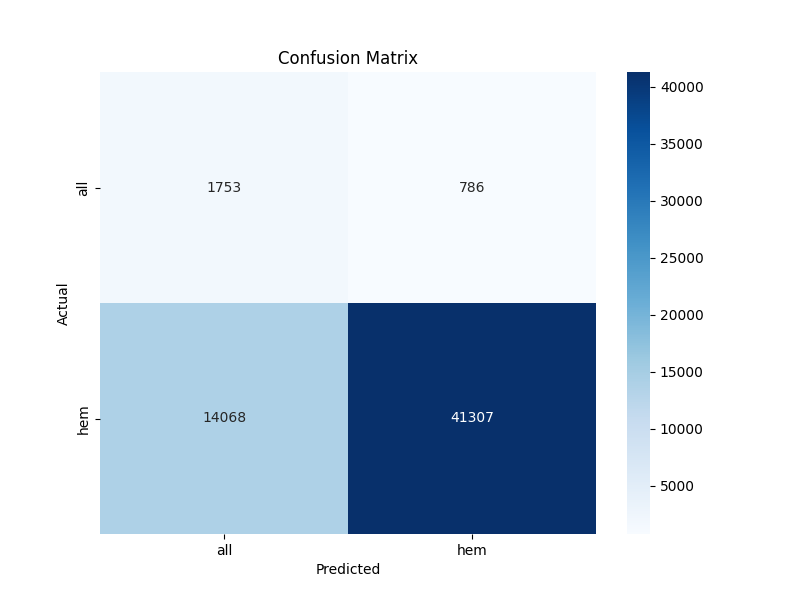
\includegraphics[width=0.8\linewidth]{images/vgg16_confusion_matrix.png}
\end{center}

\subsubsection{VGG19}
\begin{center}
	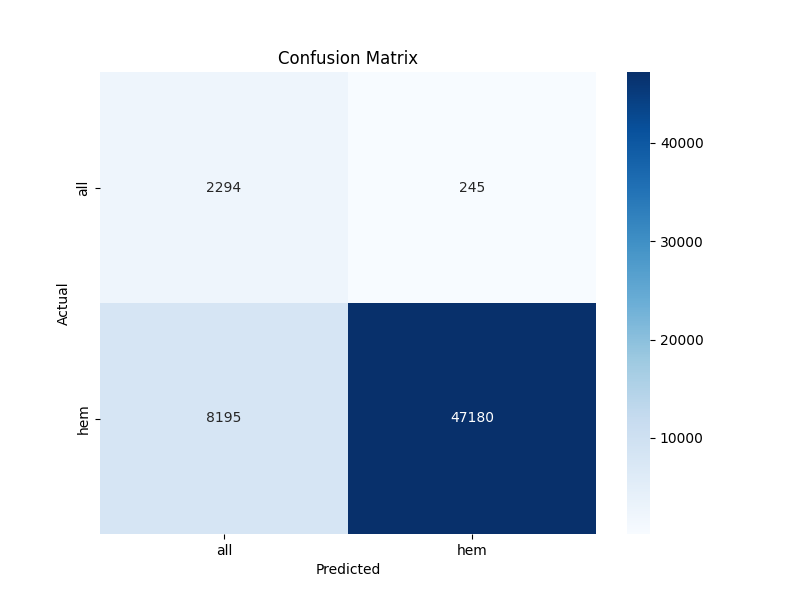
\includegraphics[width=0.8\linewidth]{images/vgg19_confusion_matrix.png}
\end{center}


\newpage
These interpretability metrics were generated with the VGG19 model

\subsubsection{Grad-CAM}

\begin{center}
	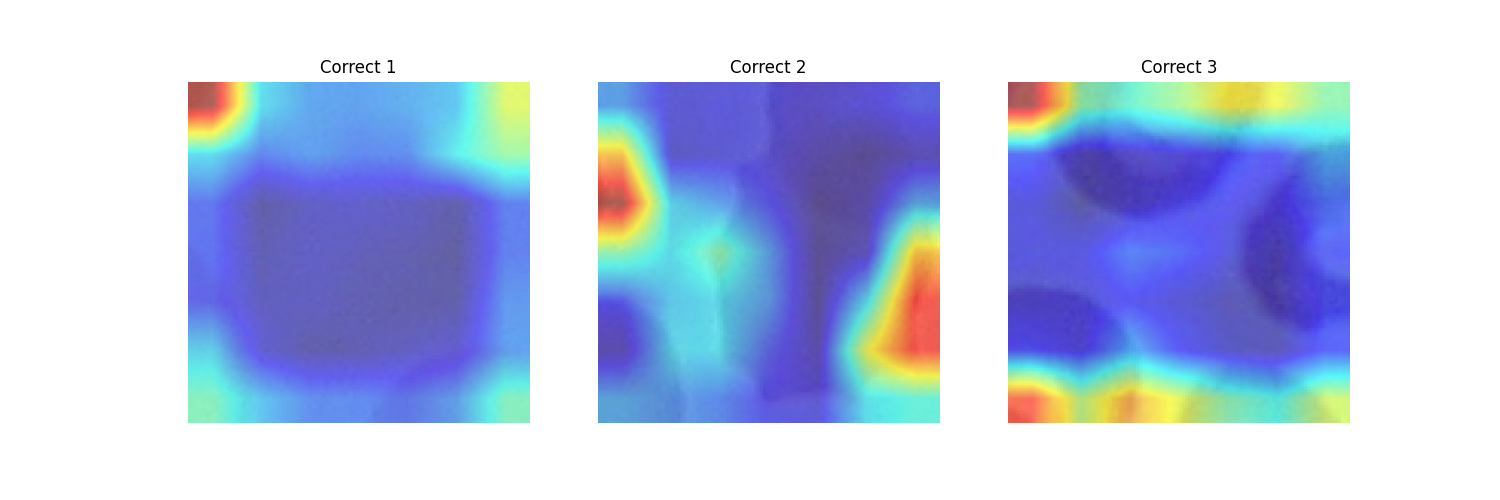
\includegraphics[width=\linewidth]{images/dataset2_gradcam_correct.png}
	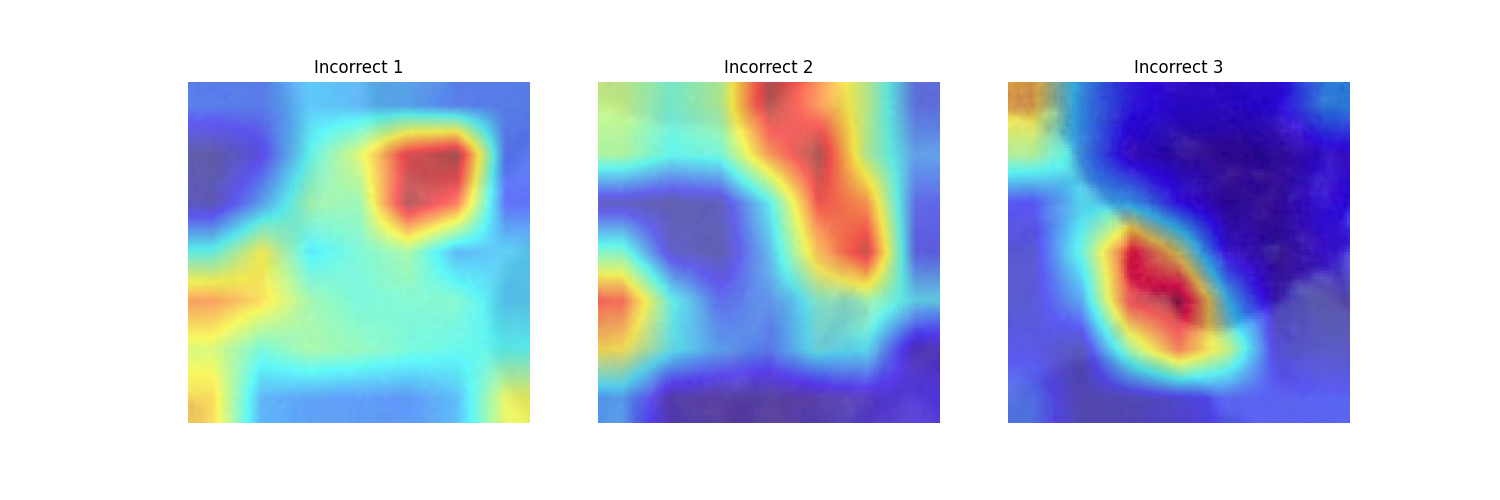
\includegraphics[width=\linewidth]{images/dataset2_gradcam_incorrect.png}
\end{center}

These images give a much more clear distinction between the correctly and incorrectly predicted images. Here it is clear in the correctly predicted images that the heatmap is focusing on the actual cells themselves whereas the heatmaps are more oriented between the cells in the incorrectly predicted images. The added complexity of the images compared to the first dataset with a single cell and solid black background has made it much easier for the model to be confused between important features and noise.

\newpage
\subsubsection{LIME}

\begin{center}
	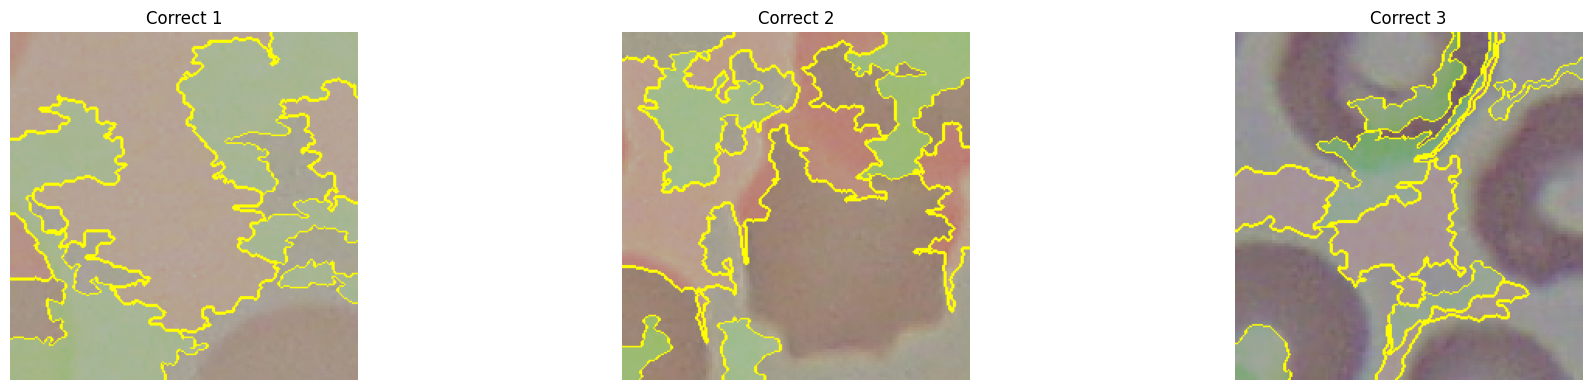
\includegraphics[width=\linewidth]{images/dataset2_lime_correct.png}
	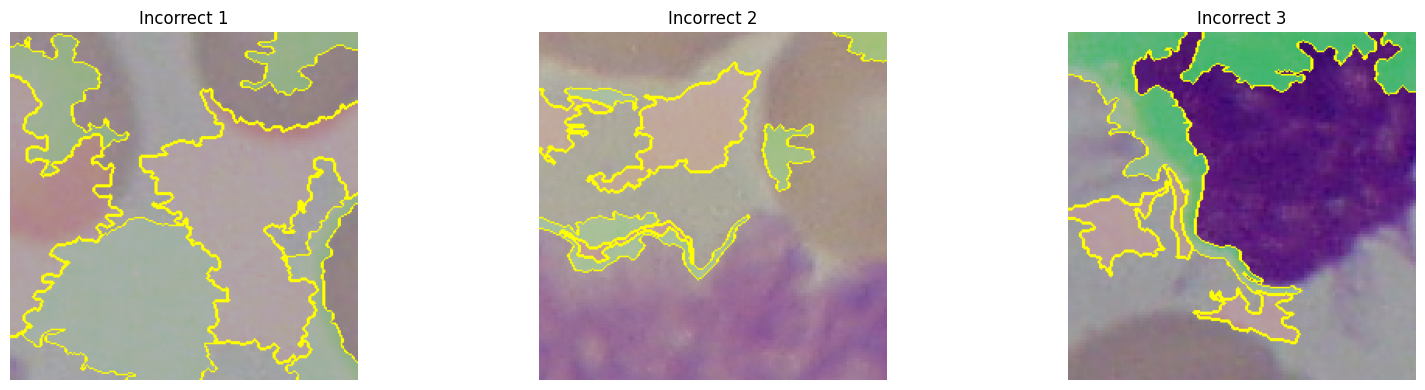
\includegraphics[width=\linewidth]{images/dataset2_lime_incorrect.png}
\end{center}

Here it is shown that the model has used a greater portion of the image to determine its outcome compared to the first dataset. While it does seem to focus more on the cells in the correctly predicted images, it isn't doing so to a significant degree so more images will need to be generated for a more accurate depiction.

\newpage
\subsubsection{SHAP}

\begin{center}
	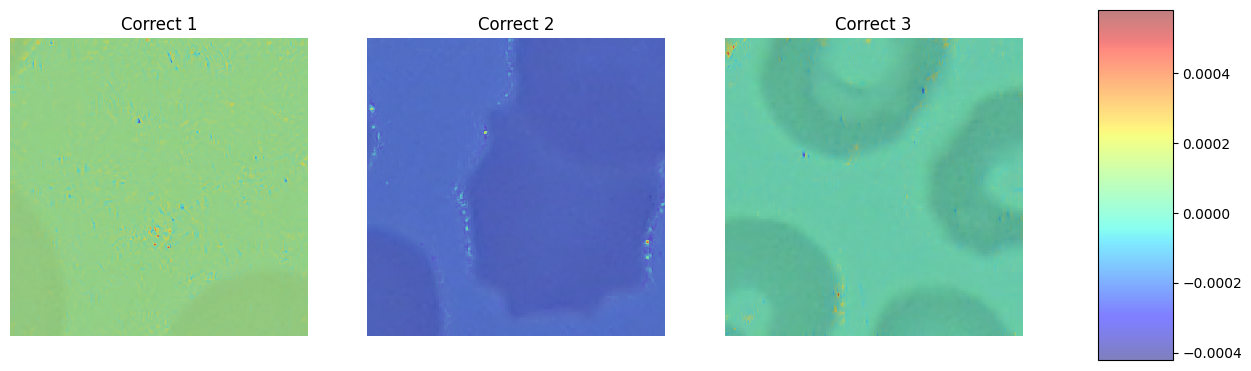
\includegraphics[width=\linewidth]{images/dataset2_shap_correct.png}
	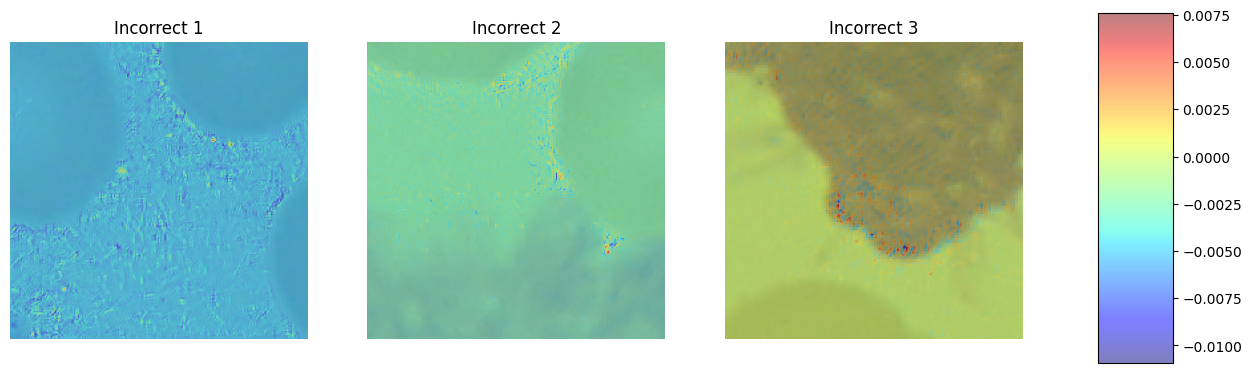
\includegraphics[width=\linewidth]{images/dataset2_shap_incorrect.png}
\end{center}

Here it is also clear how the model is using the full image to derive its outcome compared to the shapley images generated on the first dataset which only focused on the cell in the image. The incorrectly predicted images appear to have a greater contrast between the regions that are leading to higher and lower predictions with more redder reds and blues blues in the image compared to correctly predicted images which have more pixels closer to the 0 score.

\twocolumn
%------------------------------------------------

\section{Discussion}
\vspace{-1mm}
In this study, the evaluation of different deep learning models was conducted on two distinct datasets. The results from C\_NMC\_2019 underscored the superior performance of VGG models, with VGG16 and VGG19 achieving the highest metrics across accuracy, precision, recall, and F1 score. Specifically, VGG16 attained an accuracy of 0.9316 and an F1 score of 0.9335, while VGG19 reported an accuracy of 0.9189 and an F1 score of 0.9188. In contrast, other models like ResNet and DenseNet, despite their architectural depth, did not significantly outperform the VGG models. For instance, DenseNet161, one of the more complex models evaluated, achieved an accuracy of 0.8303 and an F1 score of 0.8369, falling short of the results achieved by the VGG models. Furthermore, as two variations of each model architecture was assessed, it was shown that the added layers in each model did not lead to significant improvements in results in the first dataset each within 2 percent of each other.

The findings from the ALL\_IDB1 window slides dataset provided further insights, particularly that the performance of the first dataset did not necessarily correlate to the result in the second dataset. As the images had more noise (other cells in background, non-solid background colour between cells), the added complexity led to improved performance. For this reason, VGG16 demonstrated a notable decrease in accuracy (0.7435) compared to its performance on C\_NMC\_2019, yet it maintained a high precision of 0.9432. Meanwhile, VGG19 consistently showed robust performance, mirroring its accuracy (0.9189) and F1 score (0.9188) from the first dataset. This consistency in VGG19's performance, irrespective of the dataset, highlights its reliability and adaptability.

Regarding the application of interpretability models; their utility was limited in the context of the first dataset. This limitation can be attributed to the dataset's inherent simplicity, where each image contained only a single cell. Consequently, the interpretability models did not provide substantial insights into the decision-making process of the neural networks. In contrast, when applied to the second dataset, which more accurately represents real-world data derived from minimally processed blood smear images, the interpretability models proved to be more informative. These models revealed that inaccuracies in the model's predictions often stemmed from a focus on non-cellular regions. This tendency indicates a potential shortfall in the model's ability to identify and utilise the key features necessary for distinguishing between cancerous and non-cancerous cells.

The findings suggest a nuanced understanding of model selection for medical imaging tasks. While simpler models like VGG can achieve high accuracy and generalizability, the addition of complexity in the form of deeper networks does not inherently guarantee enhanced performance. Furthermore, the effectiveness of interpretability tools appears to be highly contingent on the complexity and nature of the dataset, offering greater utility in scenarios that closely resemble real-world conditions.

%------------------------------------------------

\section{Future Work}

There are still several promising directions to enhance the performance and understanding of deep learning models in this field. Firstly, results from previously mentioned papers such as from the C\_NMC\_2019 competition have shown highly competitive results with more custom deep learning models, as these models might offer novel approaches and techniques that could be beneficial.

Another area of interest is to move beyond the conventional sliding window approach for patch processing and training an object detection model that can accurately centre each cell in an image, which could potentially improve the performance of the classification model by providing more focused and relevant input data. It would ensure the entirety of each cell is being provided to the classification model and as bounding boxes are dynamically sized, it would minimise the amount of other cells that are included in each image reducing its effect on the result.

Additionally, this study focused on applying the interpretability models on just the final layer but it is possible to apply them to other layers too. This multi-layer interpretability approach could yield more comprehensive insights into how the model processes  and transforms the data at different stages, leading to a better understanding of its behaviour and potentially guiding further improvements in the model design.

Since the primary goal of this research is to develop a model that functions as a tool for medical practitioners, it is imperative that healthcare professionals are engaged and their insights and requirements are incorporated into future model design.

%------------------------------------------------
\newpage
\section{Conclusion}
\vspace{-1mm}
This study has built off existing literature aiming to provide a competitive model in diagnosing acute leukaemia combined with comprehensive model insight. This was achieved by training various models; ResNet(50 and 101), DenseNet(121 and 161) and VGG(16 and 19) on the C\_NMC\_2019 competition dataset composed of over ten thousand cell images from a diverse group of subjects. After using several preprocessing techniques and splitting the dataset into 64\% training / 16\% validation / 20\% testing, the models were trained and compared in accuracy, precision, recall and F1 score. This resulted in VGG16 as the top performing model achieving the highest accuracy of 0.9316, precision of 0.9369, recall of 0.9301, and an F1 score of 0.9335. VGG19 followed closely, with a competitive performance showcasing an accuracy of 0.9189, albeit with marginally lower precision and recall rates. While the deeper models did perform slightly better than their less complex counterparts, they were still with 1-2 percent differences. Interestingly VGG16 managed to outperform VGG19 in every metric.

After training the models, VGG, the top performing model class, was further applied to a modified version of the ALL\_IDB1 dataset which, concentrated with the first dataset which were just images of single cells, is a dataset of full blood smear images. This dataset also contains the locations of the centroids of each blast cell in the image so sliding windows were created for patch processing.

Here, the added depth of VGG19 was advantageous leading to it outperforming VGG16 achieving an accuracy of 0.9189, precision of 0.9206, recall of 0.9189, and an F1 score of 0.9188. In contrast, VGG16 demonstrated lower efficacy with an accuracy of 0.7435, despite a notably high precision of 0.9432, which did not proportionally translate to recall, mirroring the accuracy at 0.7435, and culminating in an F1 score of 0.8188. 

Three interpretability models were applied to the top performing model of each dataset including Grad-CAM, LIME and SHAP which provided more model insight. While there was little difference between the insights in The correctly and incorrectly predicted images in the first dataset, this was likely due to the images having less noise to distract the model as each image only included a single cell and solid black background unlike real world conditions. In the second dataset however, there were more noteworthy differences between the correctly and incorrectly predicted images as the model focused less on the actual cells in the image and more on the background between them when it incorrectly predicted the image class.

Overall, the findings from this study advocate for a nuanced approach to model selection, emphasising the importance of considering dataset characteristics and the intended application environment. The remarkable performance of the VGG19 model across the evaluations positions it as a promising tool for medical practitioners, albeit with a recommendation for continued refinement and validation in diverse real-world settings. This research lays a foundation for future exploration and development of deep learning-based diagnostic tools, paving the way for more accurate, efficient, and reliable medical imaging solutions.

%------------------------------------------------

\section{Code Availability}

The source code for the machine learning models and analysis presented in this paper is available under the GNU General Public License v3 (GPLv3). The code repository additionally includes the pretrained weights of the vgg19 model along with instructions for obtaining the two datasets and how to train and run the models. It can be freely accessed at \url{https://github.com/AAbignano/ml\_leukaemia\_classification}.

%----------------------------------------------------------------------------------------
%	 REFERENCES
%----------------------------------------------------------------------------------------

\newpage

\nocite{*}

\bibliographystyle{plainnat}
\bibliography{references}

%----------------------------------------------------------------------------------------

\end{document}
